%!TEX root = ../main.tex

\begin{figure*}[t]
	\vspace{-15pt}
	\centering
	\makebox[\textwidth][c]{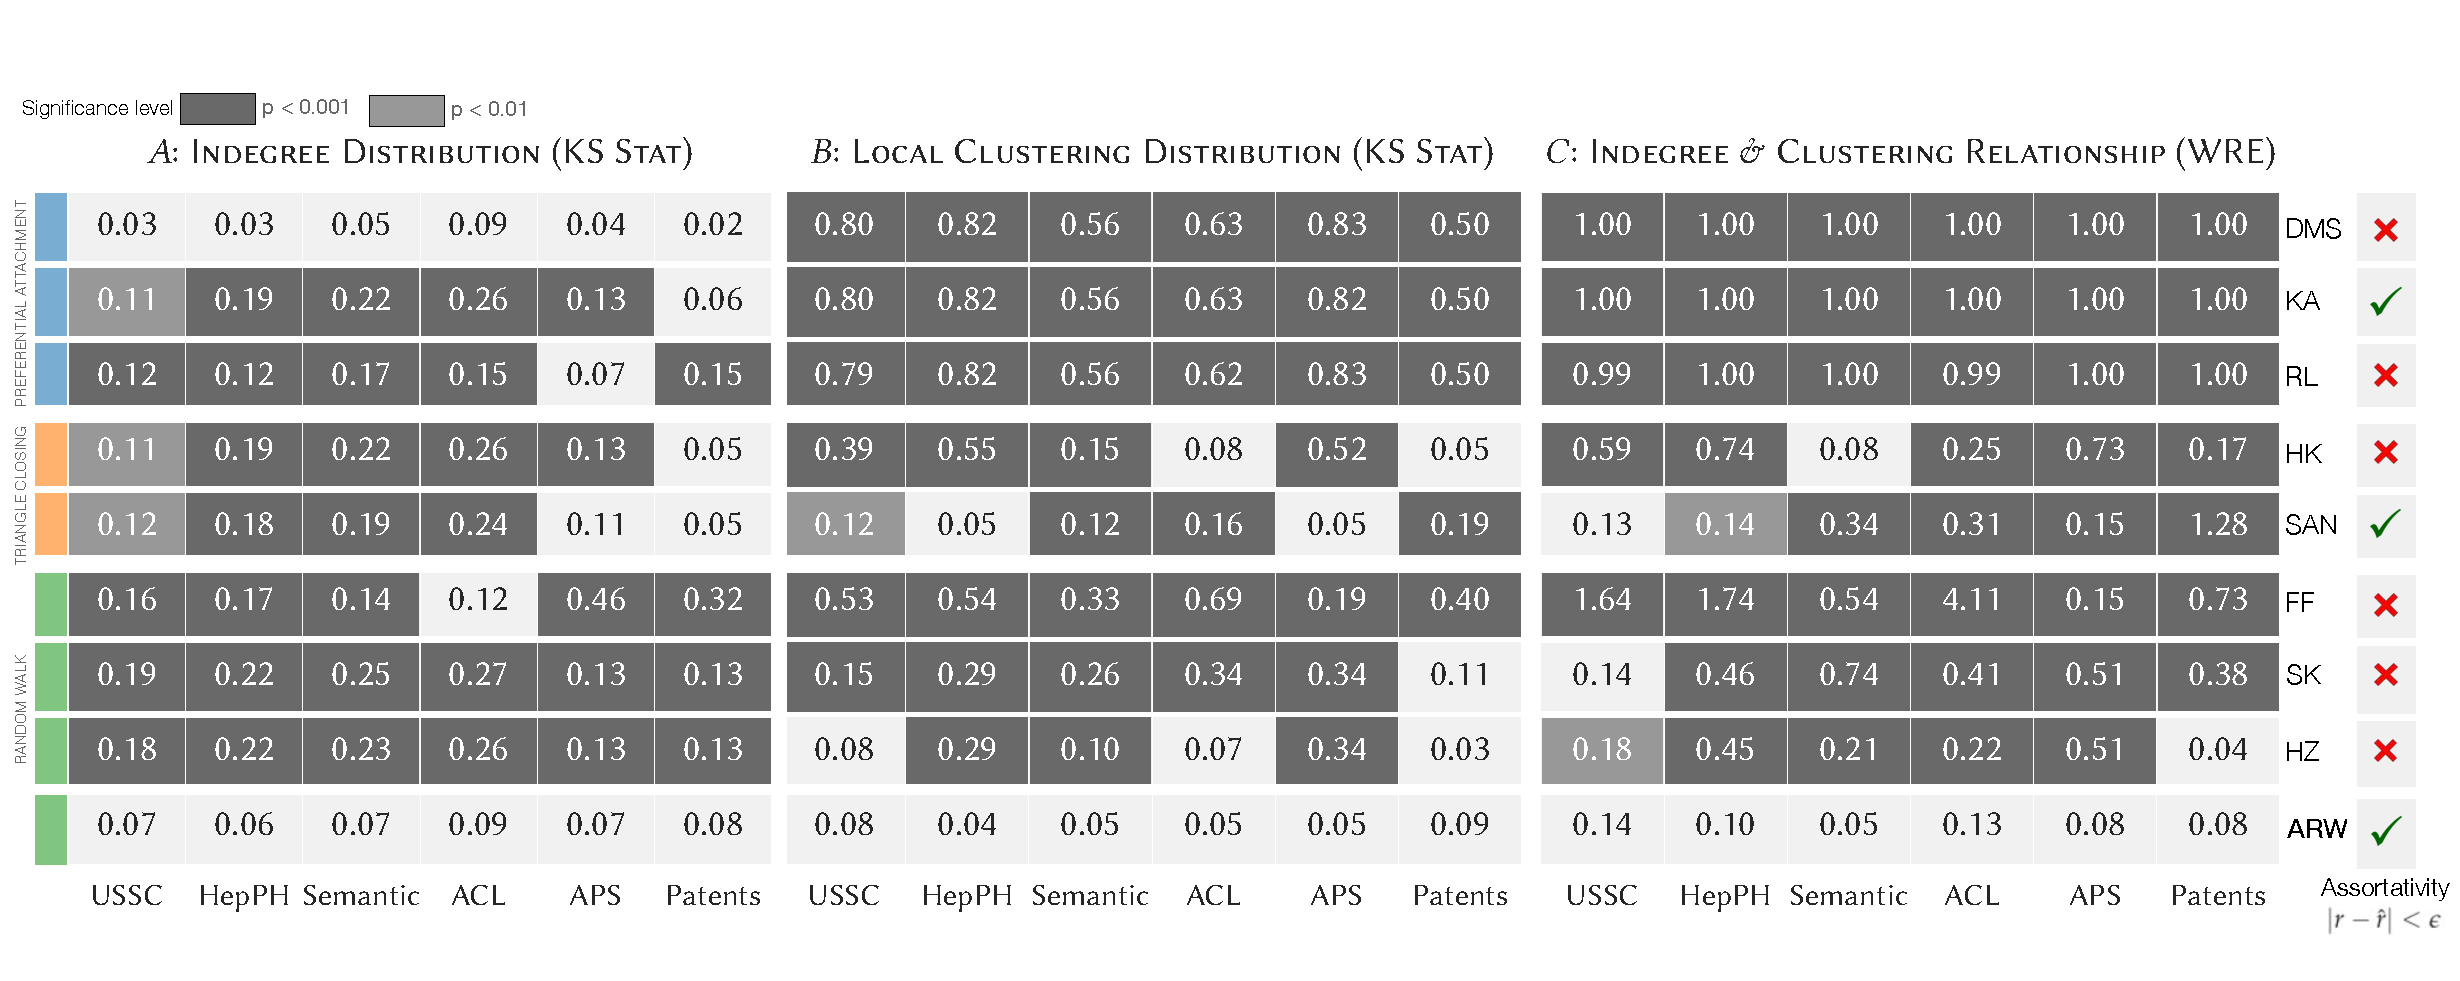
\includegraphics[width=.95\textwidth]{experiments}}
	\vspace{-16pt}
	\caption{
		Modeling network structure.
		Tables 5A, 5B and 5C
		measure the accuracy of eight models in fitting key properties of real-world networks.
		Our model, \texttt{ARW}, jointly preserves all four properties accurately and often
		performs considerably better than existing models:
		the cells are shaded gray or dark gray if the proposed model \texttt{ARW} performs
		better at significance level $\alpha=0.01$ ( \lightgraybg{ }) or $\alpha=0.001$ ( \darkgraybg{ })
		respectively.
	}
	\vspace{-13pt}
	\label{fig:exp_table}
\end{figure*}

\section{Modeling Network Structure}
\label{sec:Experiments}
In this section, we evaluate \texttt{ARW}'s efficacy in preserving
observed network structure relative to well-known growth models.

\subsection{Setup}
\label{sub:Experimental Setup}

In this subsection, we introduce eight representative growth models
and describe evaluation metrics used to fit models to the datasets.

\textit{State-of-the-art Growth Models}. We compare \texttt{ARW} to eight
models representative of the key edge formation
mechanisms: preferential attachment, fitness, triangle closing and random walks.
Two of the eight models account for attribute homophily and preserve attribute mixing patterns,
as listed in~\Cref{table:models}.
\begin{table}[t]
 \center
 {
  \begin{tabular}[c]{llcc} \toprule
  Model &  Abbreviation & Type & Attributed? \\ \midrule
  Dorogovtsev et al.~\cite{dorogovtsev2000structure} & \texttt{DMS} & \texttt{PA} & \xmark  \\
  Relay Linking~\cite{singh2017relay} 						  & \texttt{RL} & \texttt{PA} & \xmark  \\
  Kim-Altmann~\cite{kim2017effect} 							  & \texttt{KA} & \texttt{PA} & \cmark  \\ \midrule
  Social Attribute Network~\cite{gong2012evolution} 	  & \texttt{SAN} & \texttt{PA+TC} & \cmark  \\
  Holme-Kim~\cite{holme2002growing} 						  & \texttt{HK} & \texttt{PA+TC} & \xmark  \\ \midrule
  Herera-Zufiria~\cite{herrera2011generating} 				  & \texttt{HZ} & \texttt{RW} & \xmark  \\
  Saramaki-Kaski~\cite{saramaki2004scale} 					  & \texttt{SK} & \texttt{RW} & \xmark  \\
  Forest Fire~\cite{leskovec2005graphs} 					  & \texttt{FF} & \texttt{RW} & \xmark  \\
   \bottomrule
  \end{tabular}
  \vspace{1mm}
  \caption{
  	  We evaluate the performance of our model \texttt{ARW} relative to three preferential attachment
	  (\texttt{PA}) models, two pref. attachment \& triangle closing (\texttt{PA+TC}) models and 3 random walk (\texttt{RW}) models.
  }
  \label{table:models}
 }
 \vspace{-10pt}
\end{table}

\textit{Ensuring Fair Comparison}. To ensure fair comparison, we modify existing models in three ways.
First, for \texttt{DMS}, \texttt{SAN}, \texttt{KA} do not have an explicitly defined initial graph,
so we use initialization method used for \texttt{ARW}, described in~\cref{sub:Model Fitting}. Second, we extend
models that use constant node outdegree $m$ by increasing outdegree over time $m(t)$
using the method described in~\cref{sub:Model Fitting}. In the absence of model-specific parameter estimation methods,
we use grid search to estimate the parameters of every network model, including \texttt{ARW},
using evaluation metrics and selection criterion described below.

\textit{Evaluation Metrics}.
We evaluate the model fit by comparing four properties of ${G}$ \& $\hat{G}$:
degree distribution, local clustering distribution, degree-clustering relationship
and attribute assortativity. We use Kolmogorov-Smirnov (\texttt{KS}) statistic to compare univariate
distributions and Weighted Relative Error (\texttt{WRE}) for the degree-clustering relationship.
\texttt{WRE} aggregates the relative error between the average local clustering $c(k)$ and $\hat{c}(k)$ of nodes with in-degree $k$ in $G$ and $\hat{G}$ weighted by the fraction of nodes with indegree $k$ in $G$.

Jointly preserving multiple structural properties is a multi-objective optimization
problem.
Therefore, for each model, the selection criterion for the grid search parameter estimation method
chooses the model parameters that minimizes the $\ell^2$-norm of the aforementioned evaluation metrics.
We normalize the metrics before computing the $\ell^2$-norm
to prevent unwanted bias towards any particular metric.
We note that the parameter sensitivity of the Forest Fire (\texttt{FF}) model necessitates
a manually guided grid search method.

% \vspace{-11pt}
\subsection{Results}
\label{sub:Experimental Results}

Now, we evaluate the performance of \texttt{ARW} relative to eight
models on the datasets introduced in~\Cref{sec:Datasets}.
For every pair of model and dataset, ~\Cref{fig:exp_table} tabulates the evaluation metrics
described in ~\Cref{sub:Experimental Setup}.
These metrics are averaged over 100 runs and measure the accuracy with which the fitted models
preserve key global network properties: degree distribution, local clustering distribution,
degree-clustering relationship and attribute assortativity.


We use one-sided permutation tests \cite{good2013permutation} to evaluate the relative
performance of \texttt{ARW}. If \texttt{ARW} performs better than a model on a dataset
with significance level $\alpha=0.01$ or $\alpha=0.001$, the corresponding cells in~\Cref{fig:exp_table}
are shaded gray ( \lightgraybg{ }) or dark gray (~\darkgraybg{ }) respectively.
We also group models that have similar edge formation mechanisms by color-coding the
corresponding rows in~\Cref{fig:exp_table}.  We use green ticks in~\Cref{fig:exp_table} to
annotate models that preserve attribute assortativity up to two decimal places.

Existing models fail to \textit{jointly} preserve multiple properties
because they either do not account for triadic closure and homophily
or are not flexible enough to generate networks with tunable structural properties.
Preferential attachment models---\texttt{DMS}, \texttt{RL}, \texttt{KA}---preserve in-degree
distributions (\Cref{fig:exp_table}A) but not clustering because they do not account for triadic closure
(\Cref{fig:exp_table}B \&~\Cref{fig:exp_table}C).
Models that use triangle closing mechanisms---\texttt{HK}, \texttt{SAN}---lead to considerable improvement
over \texttt{DMS} and \texttt{KA} in modeling local clustering, but perform poorly w.r.t. degree-clustering
relationship.

Existing random walk models---\texttt{FF}, \texttt{SK}, \texttt{HZ}---
do not account for homophily and attribute mixing patterns.
\texttt{FF}, in particular, considerably overestimates local clustering because of its recursive edge
formation process.

\begin{figure}
	\centering
	% \vspace{-3pt}
	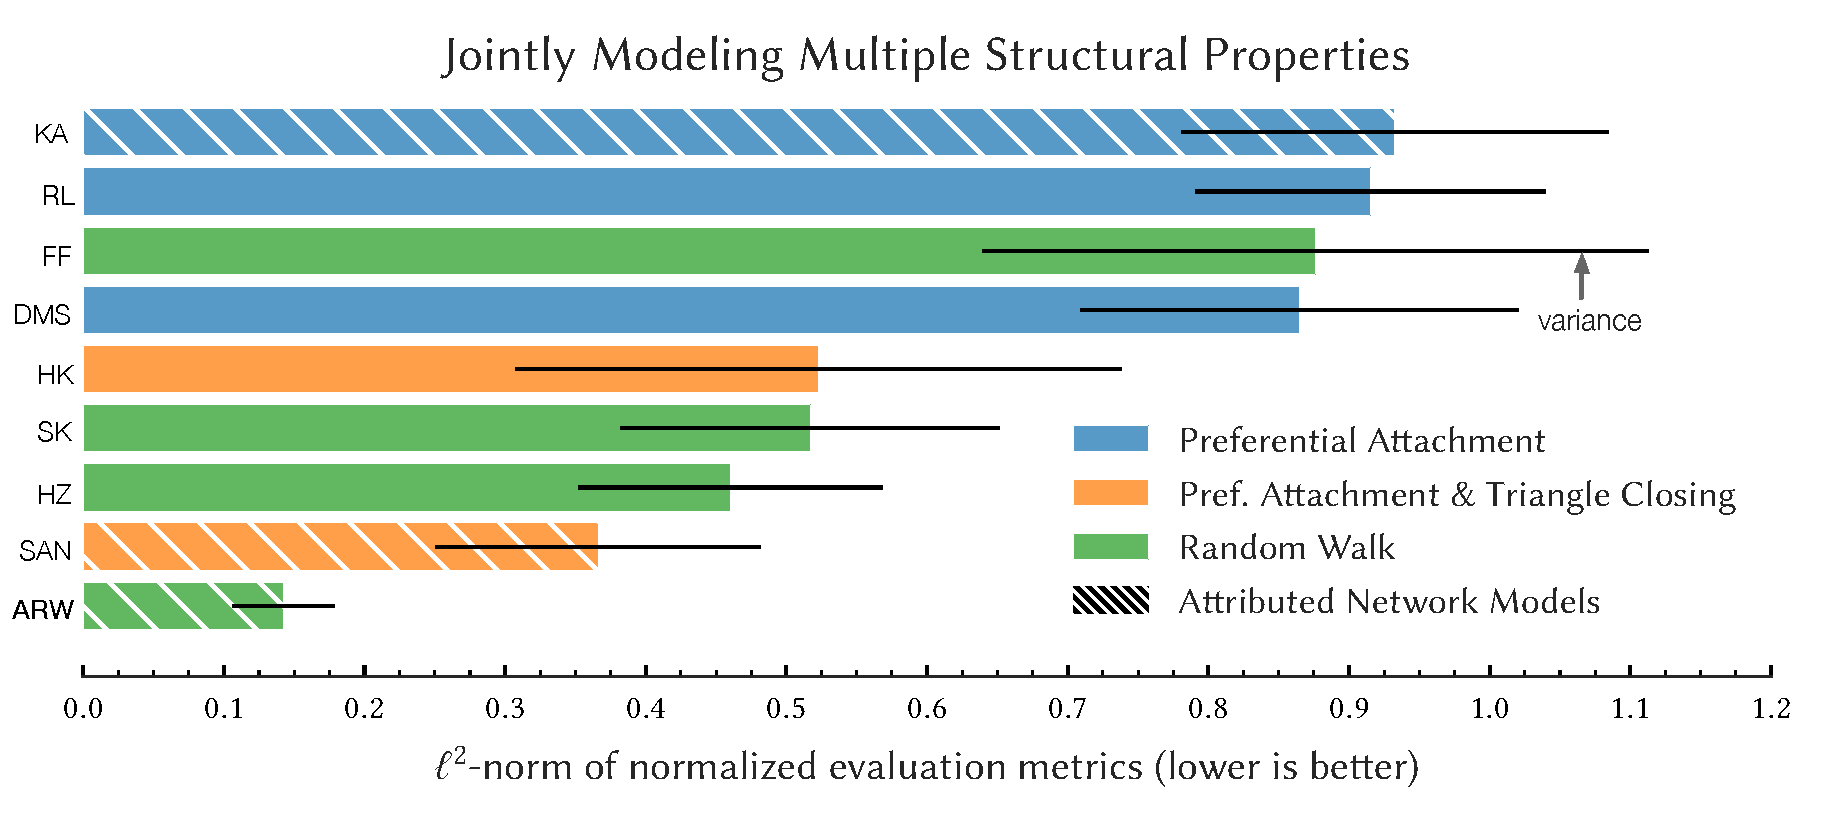
\includegraphics[width=\linewidth]{experiments_barplot}
	% \vspace{-10pt}
		\caption{\texttt{ARW} outperforms
			existing models in jointly preserving key structural properties of node in-degree
			and local clustering by a significant margin of 2.5x-10x.
		}
		\label{fig:barplot}
		\vspace{-14pt}
\end{figure}

~\Cref{fig:exp_table} clearly indicates the effectiveness
of \texttt{ARW} in {jointly} preserving multiple
global network properties. \texttt{ARW} preserves observed
in-degree distributions by adjusting nodes' bias towards high degree nodes
using $\pout$.
\texttt{ARW} matches the local clustering
distribution  (\Cref{fig:exp_table}B) and in-degree \& clustering relationship
(\Cref{fig:exp_table}C) with high accuracy using $\pjump$ and
$\plink$. \texttt{ARW} also preserves attribute assortativity using
the attribute parameters $\psame$ and $\pdiff$.

To summarize, \texttt{ARW} unifies sociological phenomena into a single
mechanism to jointly preserve key network properties significantly
better than existing models, as shown in~\Cref{fig:barplot}.
Code pertinent to \texttt{ARW} is available online \footnote{Code: https://github.com/CrowdDynamicsLab/ARW}.
Please refer to the extended version of
our paper \cite{shah2017growing} for
more information.
